\documentclass[12pt,letterpaper]{article}

\usepackage{bargar}
\usepackage{euler}
\usepackage{mathpazo}
\usepackage{amsmath}
\usepackage{graphicx}
\usepackage{amsmath}
\usepackage{fixltx2e}

\assignment{Heat Exchanger Design}
\student{Joshua Holbrook}
\duedate{May 1\textsuperscript{st} 2010}
\coursename{Thermal Systems Lab}
\coursenumber{ME 415}

\begin{document}
\sffamily

\section{Introduction \& Background}

For this exercise, we are presented with the following scenario: A rural Alaskan village has a large diesel generator. Because diesel fuel is at a premium, the operators wish to reuse the waste heat from the generator to heat a small building, namely a laundromat. Our task, then, is to design a heat exchanger to dump the waste heat from the generator into a glycol heating system. The temperature differential for the building heat is specified to be \(> 20^o F\), the minimum coolant temperature for the generator is specified at \(140^o F\), and typical operating temperatures and flow rates for the generator are given in a table.  The fluids for both sides of the heat exchanger are assumed to be 50\% by volume ethylene glycol.

\section{Mathematics \& Approach}

The basis of this analysis is the Log Mean Temperature Difference method, or LMTD method, which relies on the relation in equations \ref{eq:lmtd}, \ref{eq:cpdt} and \ref{eq:lmtd_def}, where \(T_i\) is the ith temperature, \(A_s\) is the surface area over which heat transfer is occuring, and \(U\) is the total heat transfer coefficient for the apparatus.

\begin{align}
\label{eq:lmtd}
\dot{Q} &= UA_s F(\textrm{LMTD})\\
\label{eq:cpdt}
        &= \dot{m}c_P \Delta T_{\textrm{hot}}
\end{align}

\begin{equation}
\label{eq:lmtd_def}
\textrm{LMTD} = 
\frac{ (T_{\textrm{hot, in}} - T_{\textrm{cold, out}} ) -
       (T_{\textrm{cold, in}} - T_{\textrm{hot, out}})
     }{
\log\left( 
    (T_{\textrm{hot, in}} - T_{\textrm{cold, out}} )
    \middle/ 
    (T_{\textrm{cold, in}} - T_{\textrm{hot, out}}) 
    \right) }
\end{equation}

In this case, the LMTD is defined as with the case of a counter-flow heat exchanger.  In this analysis, however, I am assuming a cross-flow heat exchanger, which requires a correction factor \(F\) to be used. This correction factor is a function of all four inlet/outlet temperatures, as well as the particular geometry of the heat exchanger.  For this analysis, the relations encoded in Cengel's Heat and Mass Transfer's graphs assuming unmixed flow were used, as seen in figure \ref{fig:correction-factor}.

\begin{figure}
\center
\label{fig:correction-factor}
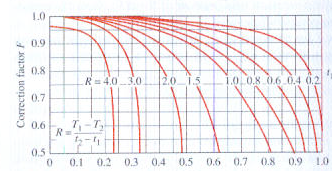
\includegraphics[width=3.0in]{correction-factor.png}
\caption{This graph shows the correction factor as a function of the derived parameters \(R\) and \(P\). Despite the low quality of the scan, the graph was still usable.}
\end{figure}

From the constraints and assumptions for this heat exchanger design, both the LMTD and \(F\) may be found.  In addition, based on the constraints for the hot side of the heat exchanger, \(\dot{Q}\) may also be calculated. With these pieces of information, we may find what the product \(UA_s\) must be in order to meet the constraints for the heat exchanger design. 

The tough part, naturally, is finding good values for \(U\) and \(A_s\). \(A_s\) is a function of the heat exchanger's geometry.  \(U\) relates to the geometry and the materials involved as in equation \ref{eq:U}, for the case of a brazed plate heat exchanger.

\begin{equation}
\label{eq:U}
U = \left(\frac{2}{h} + \frac{A_{s, \textrm{plate}} t_{\textrm{plate}}}{k_{\textrm{solid}}} \right)^{-1}
\end{equation}

This means that not only must \(A_s\) be known, but so must the thickness of the plates, the material the exchanger is made of, and the convective heat transfer coefficient across the plates, which is in turn a function of the geometry of the heat exchanger, the material properties of the fluid, and the velocity of the fluids through the exchanger.

For this design, I decided to start with pre-fabricated plates designed for brazed plate heat exchangers. This gives a good starting point for the design of the heat exchanger, removing a lot of the design variables, while still requiring the basic calculations required to actually design a heat exchanger. Moreover, while the plates might be already-designed in real life, specifications on them detailed enough to base the entire design are not easily-obtained. Therefore, basic released knowledge of plate designs will be used to make reasonable calculations for this purpose.

Due to their prominence on the Google search page, I chose to work with Schmidt's line of brazed plate heat exchangers. Figure\ref{tab:schmidt}, which depicts a table from Schmidt's literature, mostly concerns itself with dimensions. Otherwise, Schmidt reveals that the primary material for their plates is 316 stainless steel. Looking up the properties of 316 stainless steel reveals a density of \(0.29\) lbm/in\textsuperscript{3} and a heat conductivity of \(9.4\) Btu/hr/ft\textsuperscript{2}/ft/\textsuperscript{o} F .

\begin{figure}[t]
\center
\label{tab:schmidt}
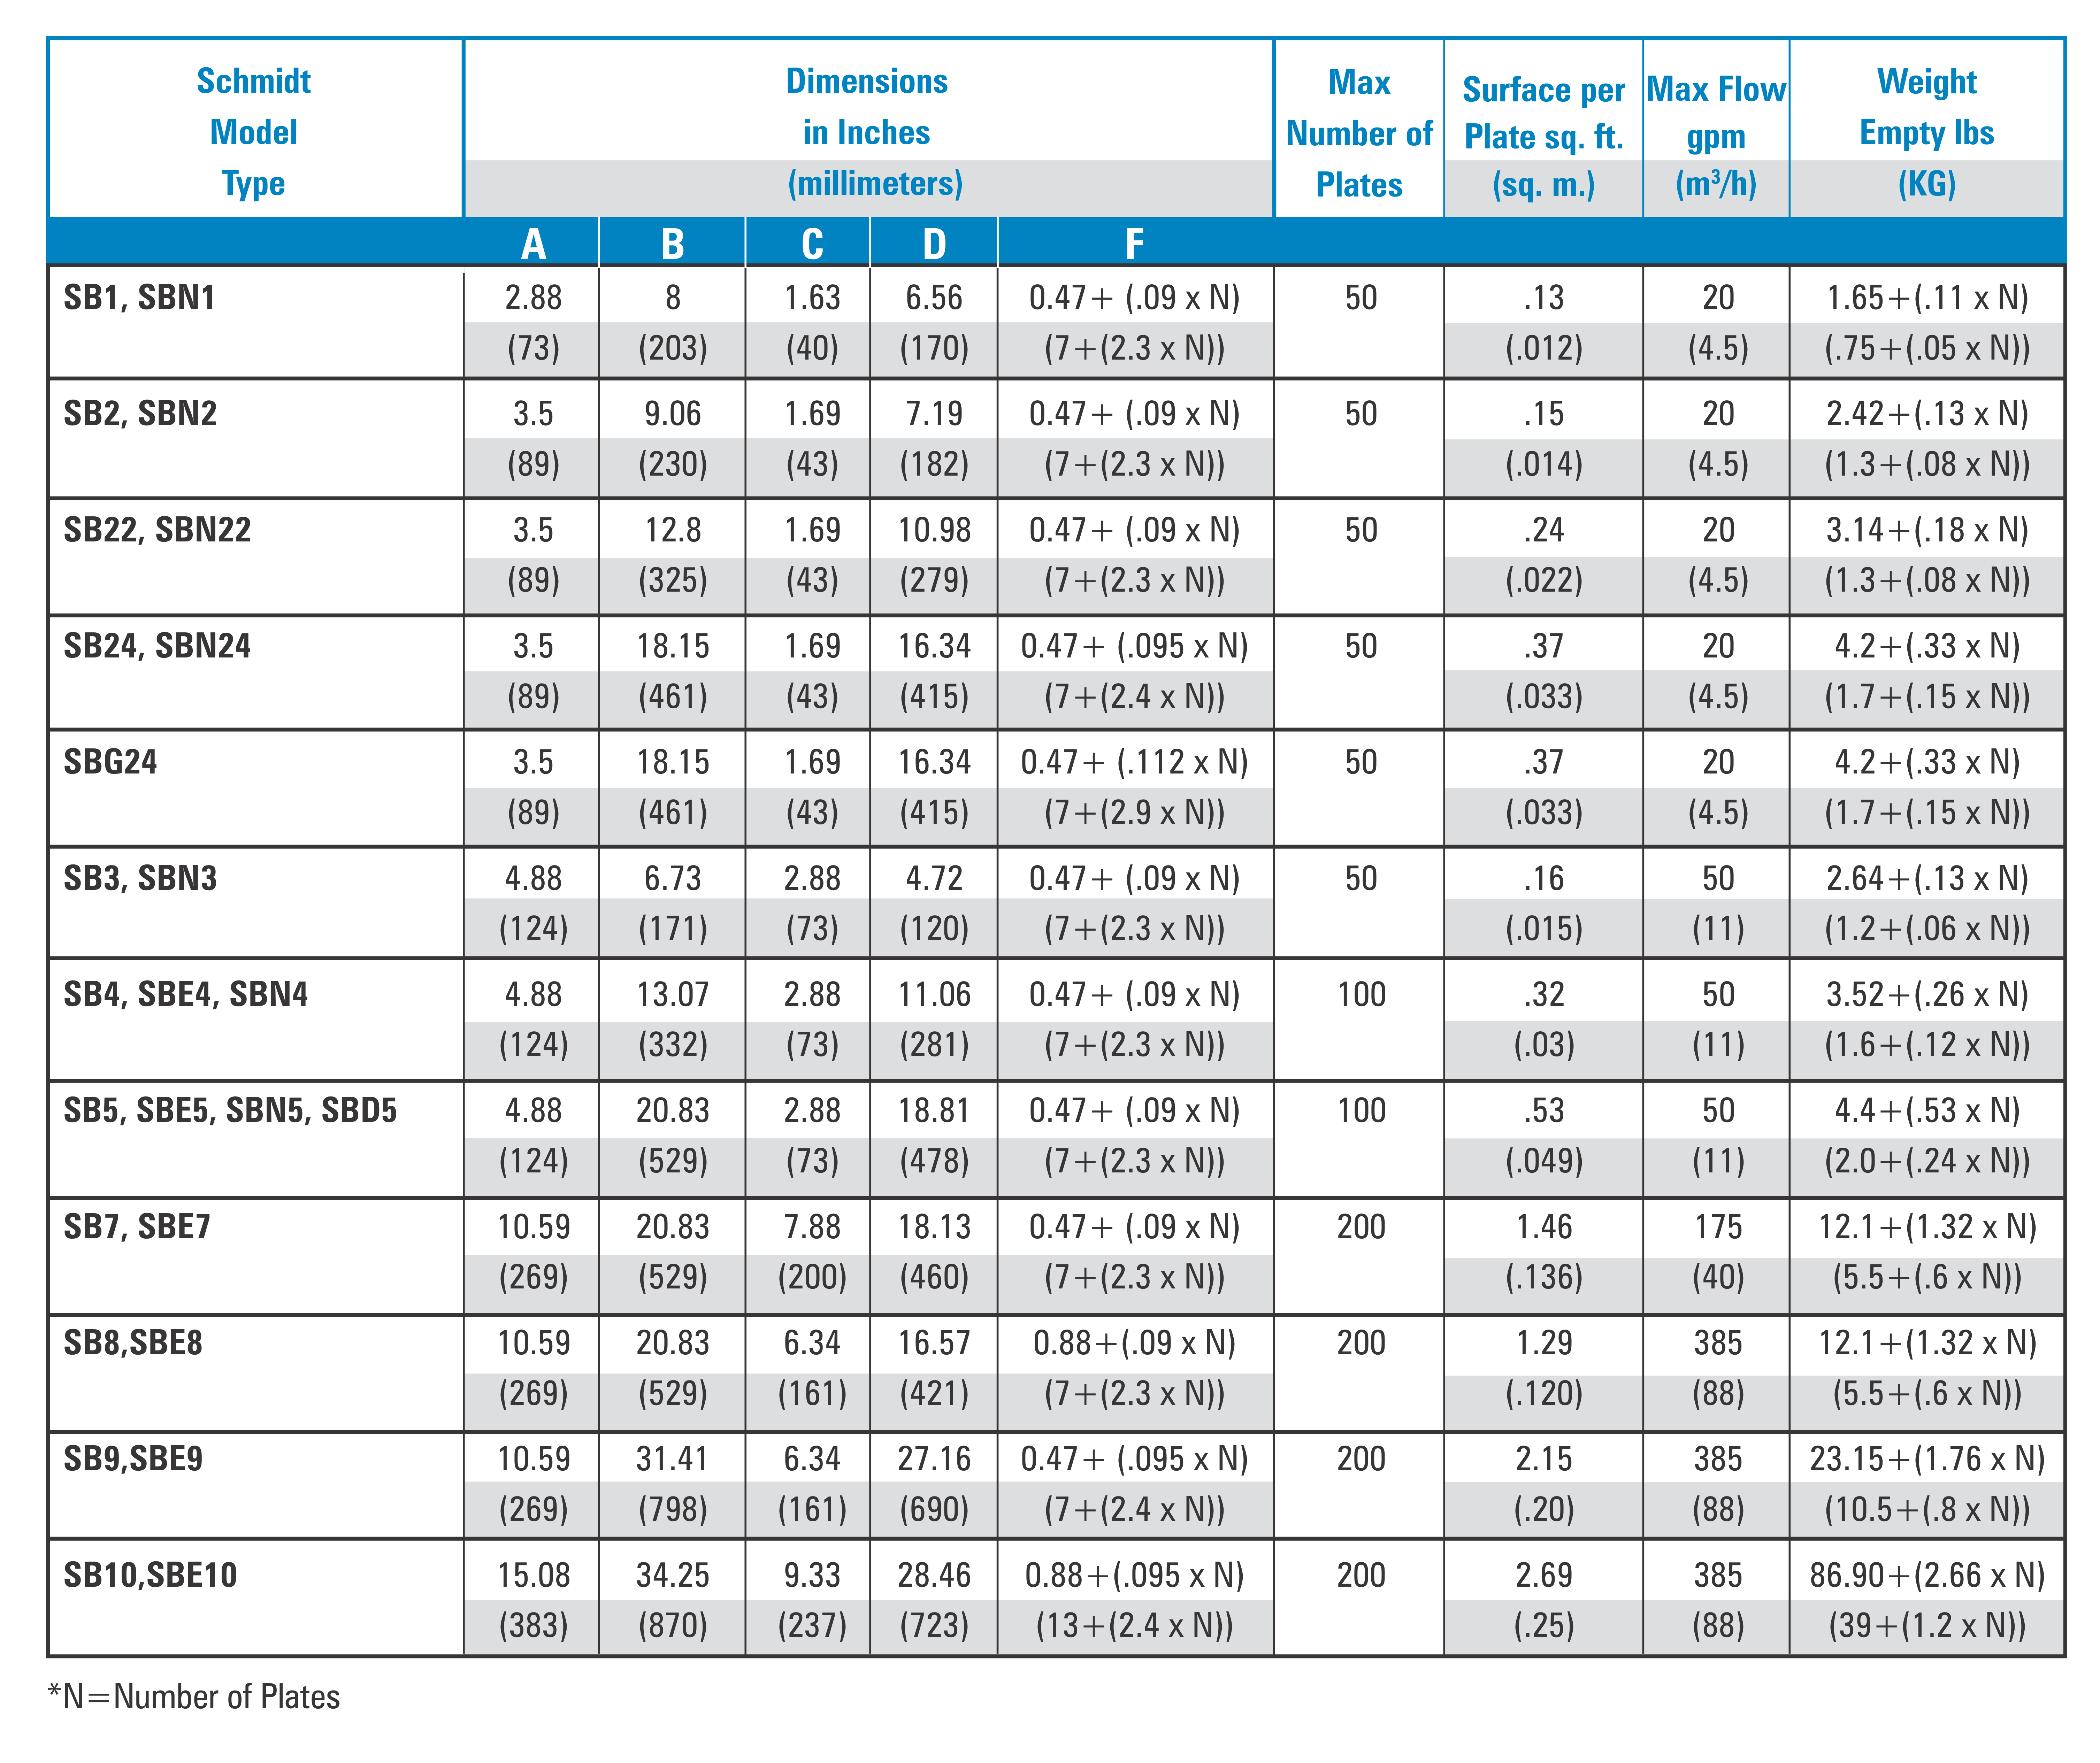
\includegraphics[width=5.0in]{schmidt_props.png}
\caption{Schmidt Brazed Heat Exchanger Properties}
\end{figure}

The average thickness of each plate may be roughly calculated as in equation \ref{eq:thickness}, where \(t_{\textrm{plate}}\) is the thickness of the plate, \(\Delta W\) is the change in weight per added plate, \(A_s\) is the surface area of one side of the plate, and \(\rho\) is the density of 316 stainless steel.

\begin{equation}
\label{eq:thickness}
t_{\textrm{plate}} = \frac{\Delta W}{\rho A_s}
\end{equation}

From this, the space between plates may also be calculated as in equation \ref{eq:spacing}, where \(\Delta l_z\) is the change in the depth of the heat exchanger per added plate.

\begin{equation}
\label{eq:spacing}
t_{\textrm{gap}} = \Delta l_z - t_{\textrm{plate}}
\end{equation}

The real-life plates are ribbed, which increases the convective heat transfer coefficients for heat transfer through the device. Unfortunately, finding these coefficients for such a complicated geometry would require computational fluid dynamics and heat transfer using a finite element method, which is out of the scope of this analysis.  Therefore, we will assume that the plates are flat, and know that the real-life convective heat transfer coefficients are significantly higher.

Assuming a flat plate, one may calculate the heat transfer coefficient using the empirical formula in equation \ref{eq:nukoverl}, where all physical properties are with respect to the fluid:

\begin{align}
\label{eq:nukoverl}
h &=\frac{k_f}{t_{\textrm{gap}}} 0.037\textrm{Re}^{0.8}\textrm{Pr}^{1/3}\\
\label{eq:re}
\textrm{Re}&=\frac{\rho v t_{\textrm{gap}}}{\mu}\\
\label{eq:pr}
\textrm{Pr}&=\frac{\mu c_P}{k}
\end{align}

As mentioned previously, finding Re requires knowing the velocity of the fluids through the heat exchanger.  The volumetric flow rate of the hot fluid, in gallons per minute, is supplied, and may be used to find the average velocity through the heat exchanger through the relation in equation \ref{eq:flow2vel}.

\begin{equation}
\label{eq:flow2vel}
v = \frac{2\dot{V}}{l_x l_z}
\end{equation}

However, the volumetric flow rate for the building heating system is unknown. However, the flow rate necessary to meet the given design constraints may be calculated, from which the velocity for the cold side may be found in a similar manner. 

Due to the first law of thermodynamics and assuming adiabatic heat transfer (which I do throughout), equation \ref{eq:firstlaw} must be satisfied.

\begin{equation}
\label{eq:firstlaw}
\left(\dot{m} c_P \Delta T \right)_{\textrm{hot}} = \left(\dot{m} c_P \Delta T \right)_{\textrm{cold}}
\end{equation}

Since all the \(\Delta T\)s are known, \(\dot{m}_{\textrm{hot}}\) may be calculated by dividing \(\dot{Q}_{\textrm{hot}}\) by \(\rho\), and \(c_P\) is a function of temperature, one may solve for \(\dot{m}_{\textrm{hot}}\), which may be converted back to \(\dot{Q}_{\textrm{cold}}\) and consequently to \(v\).

(Not that, assuming equal \(c_P\) values for both fluids, the outgoing volumetric flow rate should be roughly 25 and consequently plate sizes 1, 2, 22 and 24 may be safely ruled out.)

Referring back to equation \ref{eq:flow2vel}, notice that \(l_z\) is a function of \(N\), or the number of plates on the heat exchanger as can be seen in figure \ref{tab:schmidt}. This means that, ultimately, \(U\) and \(A_s\) are both functions of \(N\), and due to the functional nature of the material properties of the brines used, finding an analytical solution to this problem is nearly impossible.  Instead, this may be solved as a zero-finding problem. In other words, the \(N\) which satisfies this equation is the solution to equation \ref{eq:zeros}.

\begin{equation}
\label{eq:zeros}
0 = (UA_s)_{\textrm{required}} - U(N) A_s(N)
\end{equation}

Hence, given dimensions of a plate heat exchanger (with dimensions \(l_x\) and \(l_y\)) and the inlet and outlet temperatures of both the hot and the cold side, the number of plates required to achieve the required heat exchanger performance may be calculated.

\section{Data Tables}

There are four sets of data associated with this design strategy.

\subsection{Engine Coolant Data Points}

This data set consists of a series of temperature and volumetric flow rate readings from the original generator/radiator configuration. From this data, approximate probability distributions for \(T_{H, \textrm{in}}\), \(T_{H, \textrm{out}}\) and \(\dot{V}_H\) can be found (see figure \ref{fig:hists}), and based on these sensible values may be assumed for the temperatures for use in heat exchanger calculations.

\begin{figure}[t]
\center
\label{fig:hists}
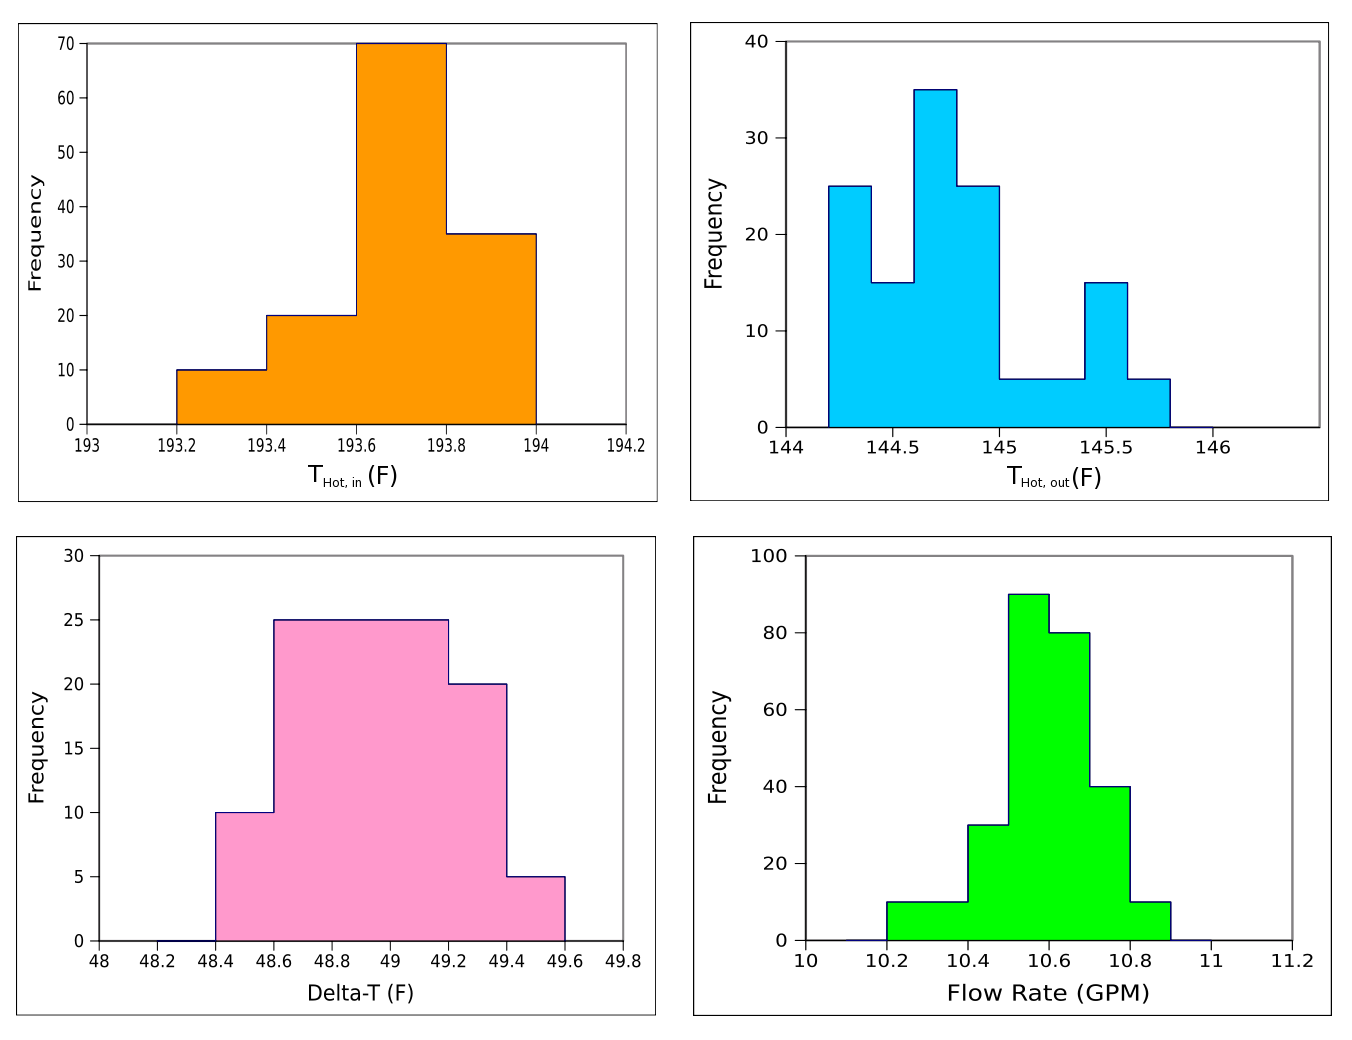
\includegraphics[width=0.8\textwidth]{histograms.png}
\caption{Histograms of the generator's run data. From the top left: The ``hot side'' of the generator loop, the ``cold side'' of the generator loop, the temperature difference between them, and the volumetric flow rate.}
\end{figure}

Another, more sophisticated approach would be to attempt some sort of stochastic approach. For example, calculations could be ran for all combinations of \(\bar{T}_i \pm \sigma_i\). Alternately, finding uncertainty equations based on those we have may be the best bet, since they could potentially decrease computer crunch time significantly. Unfortunately, such treatments of data seem to be rare enough that finding information on them is difficult. Moreover, it's a lot of effort for values that, in the case of the temperatures, tend to vary by less than a degree either way.

\subsection{50\% by volume Ethylene Glycol Property Table}

``ASHRAE 2005 Fundamentals'' contains property tables for ethylene glycol at a number of by-volume mixtures relating temperature to density, heat capacity at constant pressure, heat conductivity and dynamic viscosity all at standard pressure. For calculations, it's easiest to pick a representative temperature for the entire system at which to pull constant values for \(\rho\), \(c_P\), \(k\) and \(\mu\), but this is (of course) not technically correct. Instead, I chose the approach of looking up these values at average temperatures for the hot and cold side of the heat exchanger, respectively.

\subsection{LMTD Correction Factors}

``Heat and Mass Transfer,'' by Yunus Cengel, contains graphs relating the four inlet/outlet temperatures of a cross-flow, non-mixing heat exchanger (amongst a few other configurations) to the correction factor \(F\). Unfortunately, these values were not in table form. I converted them to table form by using a piece of open-source software called Engauge Digitizer, which is designed to convert scans of graphs into tabular form.

\subsection{Heat Exchanger Specifications Table}

Finally, the data in figure \ref{tab:schmidt}, which contains the specifications for each model of heat exchanger, was to be used for its dimension and weight values, as functions of \(N\) where applicable.

\section{Software Implementation}

The software implementation of this design, while complete enough to be worthy of discussion, is unfinished due to the complexity of the problem as posed.

As it stands, three classes were implemented to handle tabular data in .csv format:

\begin{enumerate}
\item \texttt{2dtable()} was designed to handle the correction factor tables from Cengel, which were functions of the derived values \(R\) and \(P\), both functions of the four inlet/outlet temperatures. The correction factor instance of this class allows returns \(F\) when called with \(R\) and \(P\) as arguments.
\item \texttt{Continuoustable()} was designed with the properties tables from ``ASHRAE 2005 Fundamentals'' in mind, and instances of this class return interpolated values for requested properties at a given value for the left-most property (in this case, temperature).
\item \texttt{Discretetable()}, in contrast, was designed for tables where interpolation wouldn't make sense---in particular, the engine coolant datapoints and heat exchanger parameters table. Other than the lack of value interpolation, this class has a similar structure to \texttt{Continuoustable()}.
\end{enumerate}

In addition, two other classes have been implemented:

\begin{enumerate}
\item \texttt{Tparams()} takes the four inlet/outlet temperatures as inputs and has methods returning values for LMTD\textsubscript{CF}, \(\bar{T}_H\), \(\bar{T}_C\), \(\Delta T_H\), \(\Delta T_C\), \(R\) and \(P\).
\item \texttt{Htxrparams} takes heat exchanger parameter information, with the density of steel, as inputs. It has methods returning \(t_{\textrm{plate}}\), \(t_{\textrm{gap}}\) and \(l_z(N)\).
\end{enumerate}

These two classes, supply most of the variables required to complete the rest of the mathematical calculations as explained previously

\section{Outcomes \& Conclusions}

Unfortunately, \(N\) was never actually calculated. However, this experience has delivered a number of significant outcomes. First, the method for designing a plate heat exchanger has been outlined---this is arguably the most important part conceptually. Having never approached such a problem previously, I ended up learning quite a bit about the LMTD method and how it may be used in the real world.

Second, implementation has been explored, and while one hasn't been completed the structure of an implementation has been mostly fleshed out. In addition, the use of tabular (and graphical) data with software has been studied, leading to the beginnings of what may end up being a publically-available python module (tabular.py).

In fact, not completing the calculations necessary to find \(N\) can be seen as a cautionary tale regarding simplifying assumptions (or lack thereof). For this project, I chose to make as few simplifying assumptions as I could get away with. This has the advantage of (hopefully) higher accuracy, but suffers from increased complexity. Had I made more simplifying assumptions (constant fluid properties and one model for the plates for example), I should've easily been able to calculate a value for \(N\). The moral of this project, if it has one, is this:  Make as many simplifying assumptions as you can get away with.

\end{document}
